% Document settings
\documentclass[a4paper,11pt]{article}

% Packages
  % math formulas
\usepackage{amsmath,amsthm,amssymb}
  % graphics
\usepackage{graphicx}
\usepackage{wrapfig}
  % plots
\usepackage{pgfplots}
  % other
\usepackage[warn]{mathtext}
\usepackage{cmap}
\usepackage[T1,T2A]{fontenc}
\usepackage[utf8]{inputenc}
\usepackage[english,russian]{babel}
\usepackage{icomma}

% Package settings
%% graphicx
\graphicspath{{Pictures/}}
\DeclareGraphicsExtensions{.pdf,.png,.jpg}
%% pgfplots
\pgfplotsset{width=10cm,compat=1.9}

% Title
\title{Отчет о выполнении работы №2.3.1\\Получение и измерение вакуума}
\author{Воейко Андрей Александрович, Б01-109}
\date{Долгопрудный, 2022}

% Document
\begin{document}
\maketitle
\newpage
\section{Аннотация.}
В работе измеряется объем форвакуумной и высоковакуумной частей установки, а также определяется скорость откачки системы в стационарном режиме.
\section{Теоретические сведения и экспериментальная установка.}
По степени разрежения вакуумные установки принято делить на три класса:
\begin{itemize}
        \item Низковакуумные~--- до $10^{-2}$--$10^{-3}$ торр.
        \item Высоковакуумные~--- до $10^{-2}$--$10^{-3}$ торр.
        \item Сверхвысокого вакуума~--- до $10^{-2}$--$10^{-3}$ торр.
\end{itemize}
В данной работе исследуются традиционные методы откачки механическим форвакуумным насосом до давления $10^{-2}$ торр и диффузионным масляным насосом до давления $10^{-5}$ торр, а также методы измерения вакуума в этом диапазоне.
\subsection{Экспериментальная установка.}
Установка изготовлена из стекла и состоит из фовакуумного баллона (ФБ), высоковакуумного диффузионного насоса (ВН), высоковакуумного баллона (ВБ), масляного (М) и ионизационного (И) манометров, термопарных манометров (М$_{1}$ и М$_{2}$), форвакуумного насоса (ФН) и соединительных кранов К$_{1}$, К$_{2}$ ... К$_{6}$ (рис.~\ref{fig:img1}). Кроме того, в состав установки входят: вариатор (автотрансформатор с регулируемым выходным напряжением), или реостат и амперметр для регулирования тока нагревателя диффузионного насоса.
\subsubsection{Краны.}
Все краны вакуумной установки~--- стеклянные. Стенки кранов тонки, пробки кранов полые и составляют одно целое с рукоятками. Кран К$_{1}$ используется для заполнения форвакуумного насоса и вакуумной установки атмосферным воздухом. Во время работы установки он должен быть закрыт. Трехходовой кран К$_{2}$ служит для соединения форвакууминого насоса с установкой атмосферой. Кран К$_{3}$ отделяет высоковакуумную часть установки от форвакуумной. Кран К$_{4}$ соединяет между соьой колена масляного манометра.
\begin{wrapfigure}{r}{0.4\textwidth}
  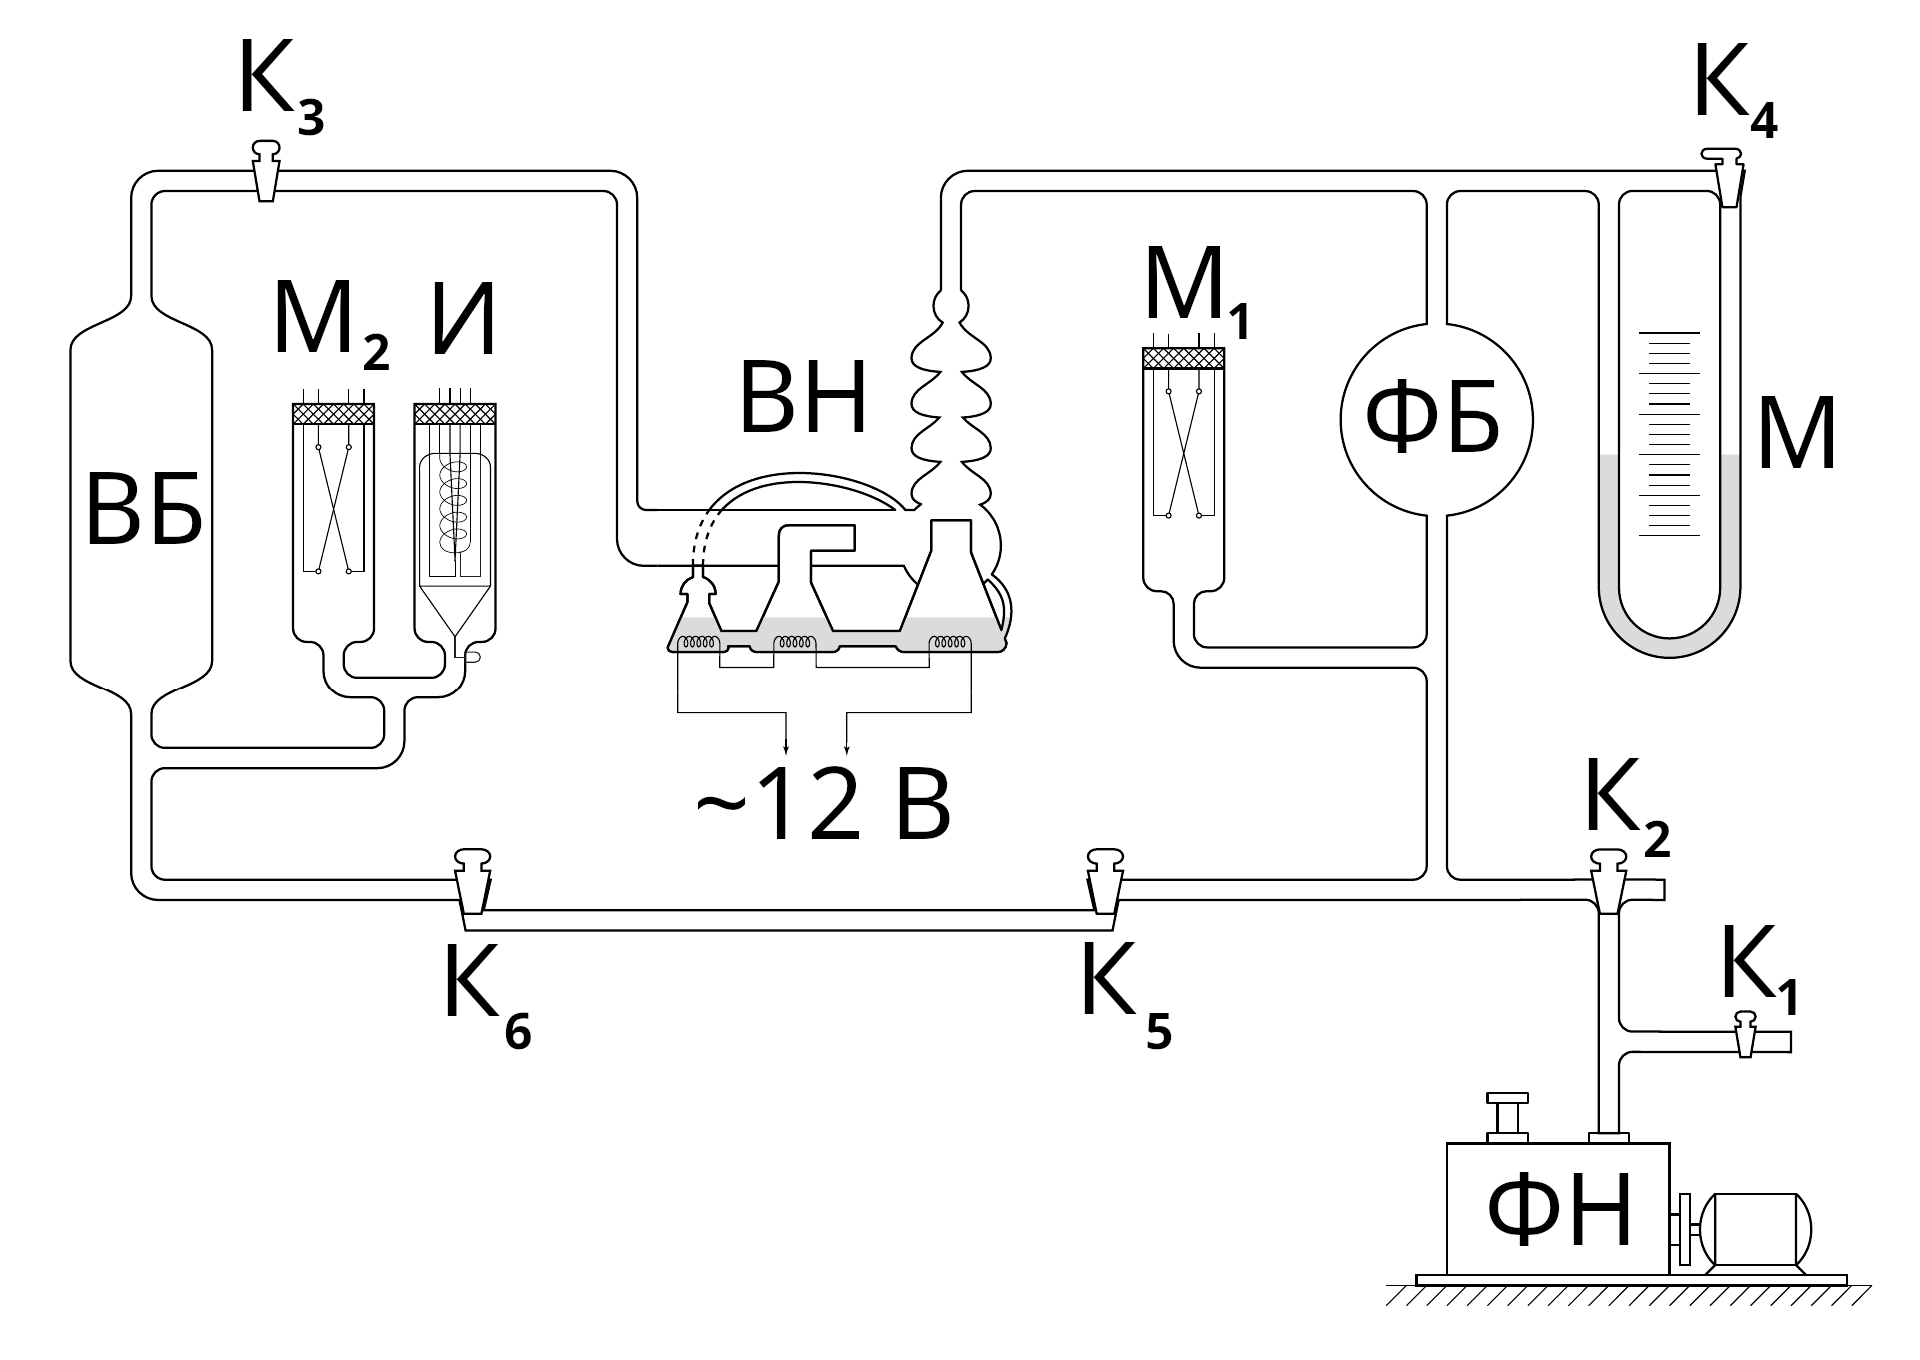
\includegraphics[scale = 0.124]{scheme1.png}
  \caption{Схема экспериментальной установки.}
  \label{fig:img1}
\end{wrapfigure}
 Он должен быть открыт во все время работы установки и закрывается лишь во время работы установки и закрывается лишь при измерении давления в форвакуумной части. Краны К$_{5}$ и К$_{6}$ стоят по концам капиояра и соединяют его с форвакуумной и высоковакуумной частями установки. Суммарный объем обоих кранов и капиляра $V_{к} = 50\ см^{3}$. Диаметр капиляра $d_{к} = 0,8\ мм$. Его длина $l_{к} = 108\ мм$.
\subsubsection{Форвакуумный насос.}
Устройство и принцип действия ротационного форвакуумного насоса, ипользующегося в данной работе, изображены на рис.~\ref{fig:img2}.\\
\begin{wrapfigure}{r!}{0.5\textwidth}
  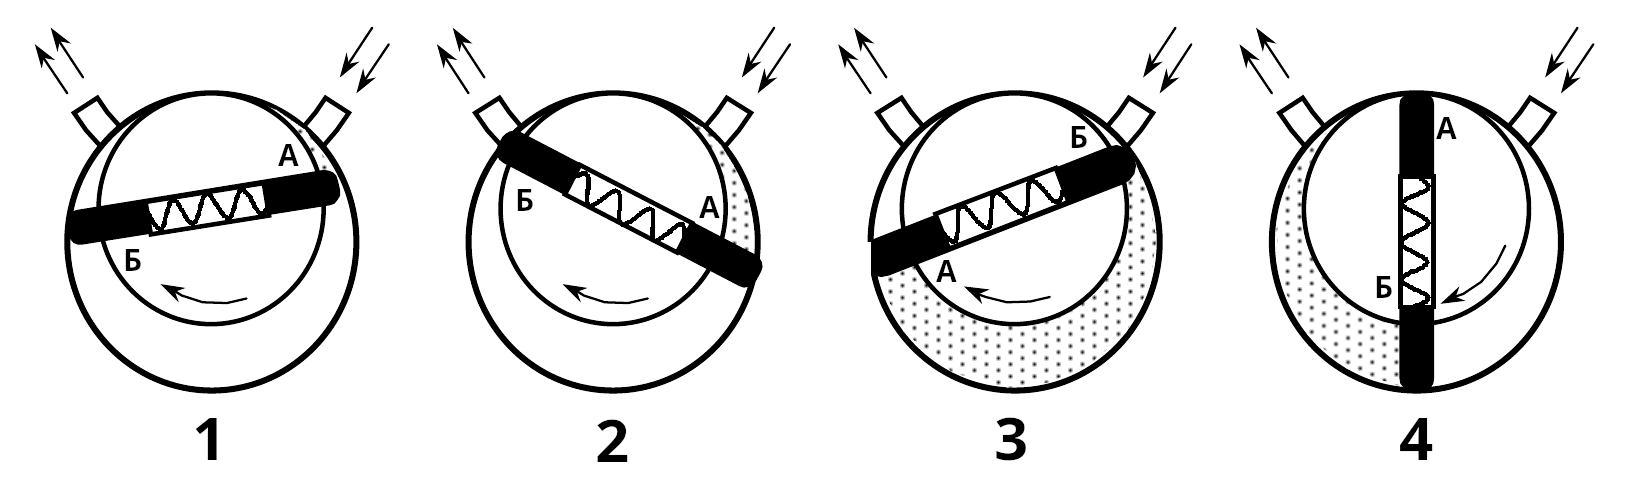
\includegraphics[scale = 0.175]{scheme2.png}
  \caption{Схема действия ротационного пластинчатого форвакууминого насоса.}
  \label{fig:img2}
\end{wrapfigure}
Насос состоит из ротора, расположенного эксцентрично в цилиндре. В роторе есть прорезь, в которой располагаются способные предвигаться в нем пластины. В ходе вращения в цилиндре образуются две полости~--- увлекаемые пластинами <<А>> и <<Б>> соответственно. На первом и втором рисунках пластина <<А>> втягивает воздух из входной трубки в полость. На третьем полость отделяется от трубки пластиной <<Б>>, а на четвертом пластина <<Б>> заталкивает воздух в выходную трубку.
\subsubsection{Диффузионный насос.}
Откасчивающее действие диффузионного насоса основано на диффузии молекул разреженного воздуха в струю паров масла. Попавшие в струю модекулы газа увлекаются ею и уже не возвращаются назад. Устройство этого насоса изображено на рис.~\ref{fig:img3}.\\
\begin{wrapfigure}{r!}{0.5\textwidth}
  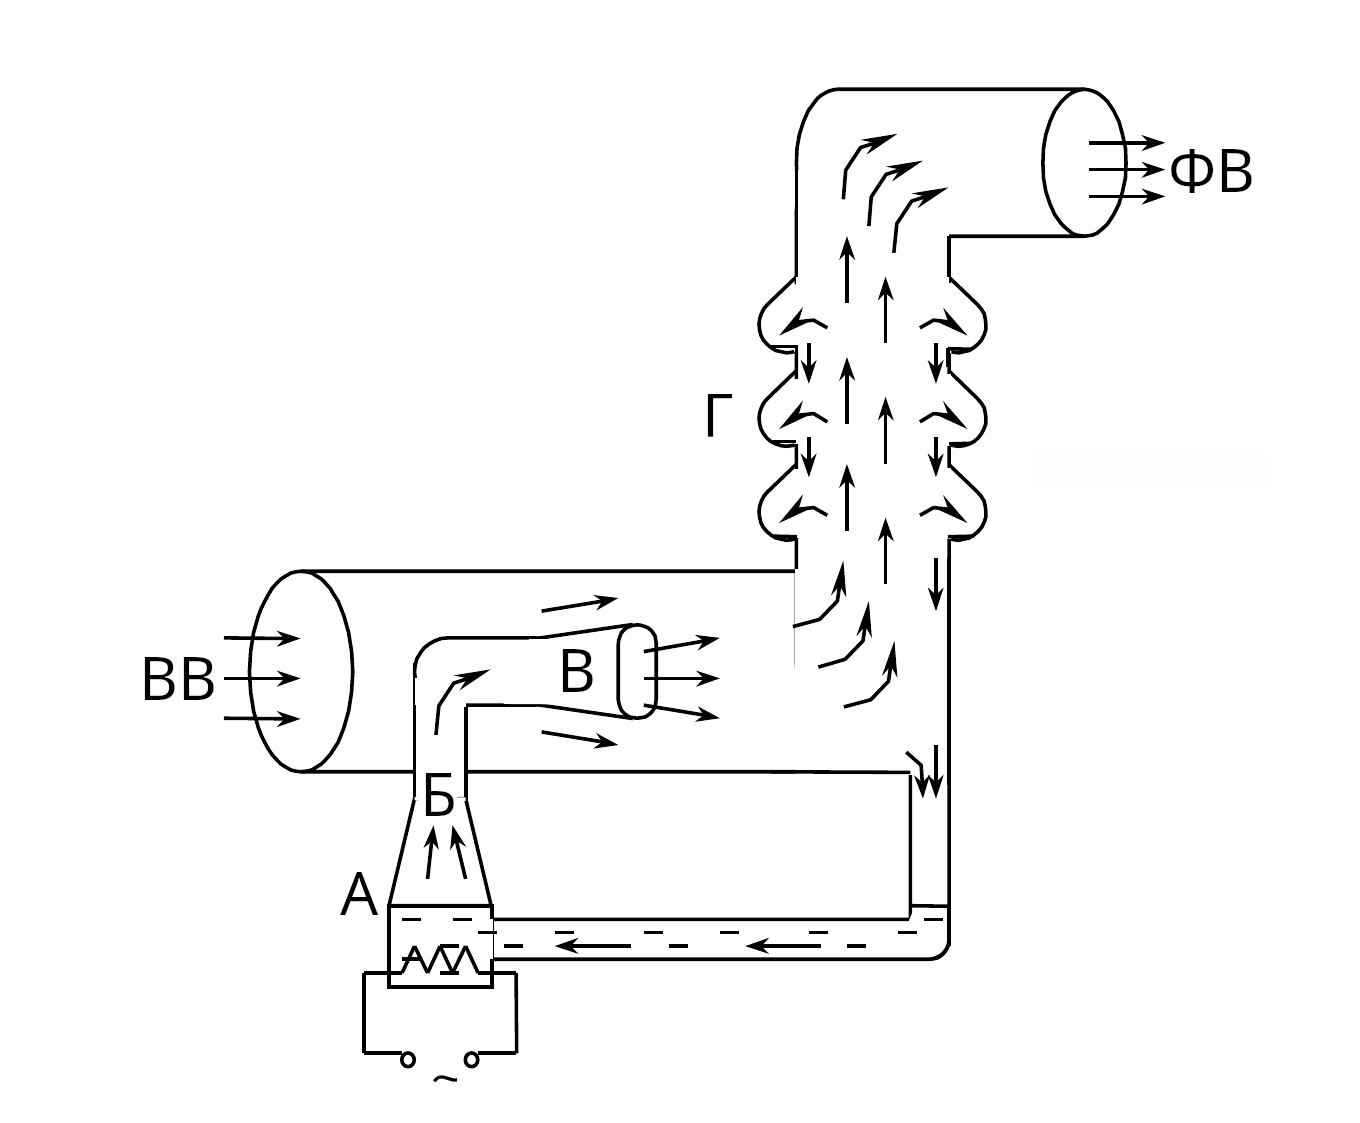
\includegraphics[scale = 0.2]{scheme3.png}
  \caption{Схема действия ротационного пластинчатого форвакууминого насоса.}
  \label{fig:img3}
\end{wrapfigure}
Масло нагревается электрической печкой. Пары масла поднимаются по трубе Б и вырываются из сопла В. Струя паров увлекает молекулы газа, которые поступают из откачиваемого сосуда через трубу ВВ. Дальше смесь попадает в вертикальную трубу Г. Здесь масло осаждается на стенках трубы и маслосборников и стекает вниз, а оставшийся газ через трубу ФВ откачивается форвакуумным насосом. Диффузионный насос работает наиболее эффективно при давлении, когда длина свободного пробега молекул воздуха примерно равна ширине кольцевого зазора между соплом В и стенками трубы ВВ. В этом случае пары масла увлекают молекулы воздуха из всего сечения зазора.
\subsubsection{Процесс откачки.}
Производительность насоса определяется скоростью откачки $W\ (л/с)$: $W$~--- это объем газа, удаляемого из сосуда при данном давлении за единицу времени. Скорость откачки фовакуумного насоса равна емкости воздухозаборной камеры, умноженной на число оборотов в секунду.\\
Рассмотрим обычную схему откачки. Разделим вакуумную систему на две части: <<откачиваемый объем>> (в состав которого включим используемые для работы части установки) и <<насос>> к которому кроме самого наоса, отнесем трубопроводы и краны, через которые производится отчкачка нашего объема. Обозначим через $Q_{д}$ количество газа, десорбирующегося с поверхности откачиваемого объема в единицу времени, через $Q_{и}$~--- количество газа, проникающего в этот объем извне~--- через течи. Будем считать, что насос обладает скоростью откачки $W$ и в то же время сам является источником газа; пусть $Q_{н}$ — поток газа, поступающего из насоса назад в откачиваемую систему. Будем измерять количество газа $Q_{д}$, $Q_{н}$ и $Q_{и}$ в единицах $PV$ (легко видеть, что это произведение с точностью до множителя $RT/\mu$ равно массе газа). Основное уравнение, описывающее процесс откачки, имеет вид:
\begin{equation}    \label{eq1}
  -VdP = \left(PW - Q_{д} - Q_{н} - Q_{и}\right).
\end{equation}
Левая часть этого уравнения равна убыли газа в откачиваемом объеме $V$, а правая определяет уоличество газа, уносимого насосом, и количество газа, уносимого насосом, и количество прибывающего вследствие перечисленных выше причин за время $dt$. При достижения предельного вакуума (давление $P_{пр}$)
$$\frac{dP}{dt}=0,$$
так что
\begin{equation}    \label{eq2}
  P_{пр}W = Q_{д} + Q_{и} + Q_{и}.
\end{equation}
Из этого уравнения найдем формулу, выражающую скорость откачки через предельный вакуум:
$$W =\left(\sum Q_{i}\right)/P_{пр}.$$
Обычно $Q_{и}$ постоянно, а $Q_{и}$ и $Q_{д}$ слабо зависят от времени, поэтому в наших условиях все эти члены можно считать постоянными. Считая также постоянной скорость откачки $W$, уравнение~\ref{eq1} можно проинтегрировать и, используя~\ref{eq2}, получить
\begin{equation}    \label{eq3}
  P - P_{пр} = \left(P_{0} - P_{пр}\right) \exp \left(-\frac{W}{V} t\right),
\end{equation}
где $P_{0}$~--- начальное давление. Оно обычно велико по сравнению с $P_{пр}$, поэтому можно записать, что
\begin{equation}    \label{eq4}
  P = P_{0} \exp \left(-\frac{W}{V} t\right) + P_{пр}.
\end{equation}
Постоянная времени откачки $\tau = V/W$ является мерой эффективности откачной системы.
Рассмотрим теперь, чем определяется скорость откачки системы. По условию эта скорость характеризует действие всей откачивающей системы, которую мы пока обохначали общим понятием <<насос>>. На самом деле эта система состоит из собственно насоса, а также из кранов и трубопроводов, соединяющих его с откачиваемым объемом.
\subsubsection{Искуственная течь.}
Для количества газа, протекающего через трубку в условиях высокого вакуума, спарведлива формула
\begin{equation}    \label{eq5}
  \frac{d(PV)}{dt} = \frac{4}{3} r^{3}\sqrt{\frac{2\pi RT}{\mu}\ }\frac{P_{2} - P_{1}}{l}.
\end{equation}
Для капилляра формула выглядит так.
\begin{equation}    \label{eq6}
  C_{капилл} = \left(\frac{dV}{dt} \right)_{капилл} = \frac{4}{3}\frac{r^{3}}{L}\sqrt{\frac{2\pi RT}{\mu}\ }.
\end{equation}
\section{Результаты измерений и обработка данных.}
\subsection{Определение объема форвакуумной и высоковакуумной частей.}
Запустим комнатный воздух в установку с открытыми кранами $К_{5}$ и $К_{6}$, а затем закроем эти краны, чтобы запереть в этом объеме $50\ см^{3}$ воздуха при атмосферном давлении.\\
Затем закроем краны, соединяющие установку с атмосферой и насосом, и включим форвакуумный насос, чтобы он откачал воздух из себя. Далее открываем кран $К_{2}$ и откачиваем установку до $\sim 10^{-2}\ торр$. После этого снова отключим установку от насоса.\\
Получившееся давление в установке равно $1,6 \cdot 10^{-2} торр$.\\
Затем, отделяем краном $К_{3}$ высоковакуумную часть установки от форвакуумной. Открываем  кран $К_{4}$ для приведения масляного манометра к готовности. Затем открываем кран $К_{5}$, и измеряем давление в форвакуумной части.\\
Высота первого столбика $h_{1} = 34,4\ см$, второго~--- $h_{2} = 9,2\ см$, давление в форвакуумной части вместе с капиляром составляет $p_{фв} = 2190\ Па$. Отсюда находим объем форваккумной части $V_{фв} = V_{к} \cdot p_{атм}/p_{фв} = 2260\ см^{3} = 2,26\ л$.\\
Далее открываем краны $К_{3}$ и $К_{6}$. После установления давления, снова измерим его манометром.
Высота первого столбика $h_{3} = 34,4\ см$, второго~--- $h_{4} = 9,2\ см$, давление в установке вместе с капиляром составляет $p_{фв + вв} = 1400\ Па$. Отсюда находим объем установки $V_{фв + вв} = V_{к} \cdot p_{атм}/p_{фв + вв} = 3530\ см^{3} = 3,53\ л$. $V_{вв} = V_{фв + вв} - V_{фв} = 1280\ см^{3} = 1,28\ л$.
\subsection{Получение высокого вакуума.}
Снова откачаем установку форвакуумным насосом. Далее включаем термопарный манометр. После того, как давление упало до уровня $p_{фв} = 0,0014\ торр$, закроем кран $К_{6}$. И начнем нагрев масла до температуры кипения. Измерим предельное давление: $p_{пр} = 1,5 \cdot 10^{-4}\ торр$. Далее отключаем откачку высоковакуумной части краном $К_{3}$. Когда вакуум испортится до давления $p_{0} = 7,9 \cdot 10^{-4}\ торр$. Далее снова включим откачку и будем записывать показания давления от времени. Результат находится в таблице~\ref{table:tab1}. Также там находится вычисленная величина $V_{вв}\ ln \left( \frac{P - P_{пр}}{P_{0}} \right)$, необходимая для построения графика с дальнейшем вычислением расхода воздуха в диффузионном насосе.
% Начало таблицы 1 {{{
\begin{table}[h!]
\centering
\begin{tabular}{ ||c|c|c|c|| }
  \hline
  № & Прошло, $с$ & $p$, $ \cdot 10^{-4}$ торр & $V_{вв}\ ln \left( \frac{P - P_{пр}}{P_{0}} \right)$, л \\
  \hline
  1 & $0,0$ & $7,9 \pm 0,1$ & $-0,27 \pm 0,02$ \\
  2 & $0,5$ & $7,8 \pm 0,1$ & $-0,29 \pm 0,02$ \\
  3 & $1,0$ & $7,7 \pm 0,1$ & $-0,31 \pm 0,02$ \\
  4 & $1,5$ & $7,4 \pm 0,1$ & $-0,37 \pm 0,02$ \\
  5 & $2,0$ & $7,1 \pm 0,1$ & $-0,44 \pm 0,02$ \\
  6 & $2,5$ & $6,7 \pm 0,1$ & $-0,53 \pm 0,02$ \\
  7 & $3,0$ & $6,2 \pm 0,1$ & $-0,66 \pm 0,02$ \\
  8 & $3,5$ & $5,6 \pm 0,1$ & $-0,84 \pm 0,03$ \\
  9 & $4,0$ & $5,0 \pm 0,1$ & $-1,04 \pm 0,03$ \\
  10 & $4,5$ & $4,4 \pm 0,1$ & $-1,27 \pm 0,07$ \\
  11 & $5,0$ & $3,9 \pm 0,1$ & $-1,52 \pm 0,07$ \\
  12 & $5,5$ & $3,5 \pm 0,1$ & $-1,75 \pm 0,07$ \\
  13 & $6,0$ & $3,1 \pm 0,1$ & $-2,03 \pm 0,07$ \\
  14 & $6,5$ & $2,8 \pm 0,1$ & $-2,30 \pm 0,07$ \\
  15 & $7,0$ & $2,5 \pm 0,1$ & $-2,63 \pm 0,07$ \\
  16 & $7,5$ & $2,3 \pm 0,1$ & $-2,92 \pm 0,07$ \\
  17 & $8,0$ & $2,2 \pm 0,1$ & $-3,09 \pm 0,08$ \\
  18 & $8,5$ & $2,0 \pm 0,1$ & $-3,52 \pm 0,09$ \\
  19 & $9,0$ & $1,9 \pm 0,1$ & $-3,81 \pm 0,11$ \\
  20 & $9,5$ & $1,8 \pm 0,1$ & $-4,17 \pm 0,2$ \\
  21 & $10,0$ & $1,8 \pm 0,1$ & $-4,17 \pm 0,4$ \\
  22 & $10,5$ & $1,7 \pm 0,1$ & $-4,69 \pm 0,7$ \\
  23 & $11,0$ & $1,7 \pm 0,1$ & $-4,69 \pm 0,7$ \\
  24 & $11,5$ & $1,6 \pm 0,1$ & $-5,58 \pm 1,0$ \\
  25 & $12,0$ & $1,6 \pm 0,1$ & $-5,58 \pm 1,0$ \\
  26 & $12,5$ & $1,5 \pm 0,1$ & --- ($\rightarrow\infty$) \\
  \hline
\end{tabular}
\caption{Результаты измерения зависимости давления от времени при улучшении вакуума.}
\label{table:tab1}
\end{table}
% }}} Конец таблицы 1
По данным измерений построим график.
% Граф. 1 {{{
\begin{center}
\begin{tikzpicture}
\begin{axis}[
    xlabel = {$t$, $с$},
    ylabel = {$V_{вв}\ ln \left( \frac{P - P_{пр}}{P_{0}} \right)$, $л$},
    xmin = -1,
    xmax = 13,
    ymin = -6.096,
    ymax = 1.947,
    grid = major,
    minor tick num = 6
]
\addplot[
    mark size=1.7pt,
    only marks,
    % only Marx,
    magenta,
]
table {
    x    y
    0    -0.27
    0.5  -0.29
    1    -0.31
    1.5  -0.37
    2    -0.44
    2.5  -0.53
    3    -0.66
    3.5  -0.83
};
\addplot[
    mark size=2.0pt,
    only marks,
    % only Marx,
    blue,
]
table {
    x    y
    4    -1.04
    4.5  -1.28
    5    -1.52
    5.5  -1.75
    6    -2.04
    6.5  -2.30
    7    -2.63
    7.5  -2.92
    8    -3.09
    8.5  -3.52
    9    -3.81
    9.5  -4.17
    10   -4.17
    10.5 -4.69
    11   -4.69
    11.5 -5.57
    12   -5.57
};
\addplot[
    mark size=1.7pt,
    no marks,
    % only Marx,
    black,
]
table {
    x    y
    -1   1.947
    13   -6.096
};
\end{axis}
\end{tikzpicture}\newline
Рис. 5: Зависимость давления от времени.
\end{center}
% }}}
Из графика видно, что примерно с 4 секунды зависимость похожа на линейную. Это связанно с тем, что в соответсвии с уравнением~\ref{eq4}:
$$P = P_{0} \exp \left(-\frac{W}{V} t\right) + P_{пр} \Rightarrow$$
$$\Rightarrow V \ln \left(\frac{P - P_{пр}}{P_{0}}\right) = -Wt.$$
До четвертой секунды процесс просто не успел полностью вступить в силу.
Аппроксимируем данные начианая с 4 секунды к прямой. Вычислив угловой
коэффицент, получаем $-W = -0,57\ л/с$, то есть $W = 0,57\ л/с$.
Теперь снова закроем кран $К_{3}$ и пронаблюдаем за ухудшением вакуума. Результаты измерений представленны в таблице~\ref{table:tab2}.
% Начало таблицы 2 {{{
\begin{table}[h!]
\centering
\begin{tabular}{ ||c|c|c||c|c|c|| }
  \hline
  № & Прошло, $с$ & $p$, $ \cdot 10^{-4}$ торр & № & Прошло, $с$ & $p$, $ \cdot 10^{-4}$ торр \\
  \hline
  1 & $0,0$ & $1,5 \pm 0,1$ & 34 & $26,0$ & $4,8 \pm 0,1$ \\
  2 & $0,5$ & $1,6 \pm 0,1$ & 35 & $26,5$ & $4,9 \pm 0,1$ \\
  3 & $3,0$ & $1,7 \pm 0,1$ & 36 & $27,5$ & $5,0 \pm 0,1$ \\
  4 & $5,0$ & $1,8 \pm 0,1$ & 37 & $28,0$ & $5,1 \pm 0,1$ \\
  5 & $6,0$ & $1,9 \pm 0,1$ & 38 & $29,0$ & $5,2 \pm 0,1$ \\
  6 & $6,5$ & $2,0 \pm 0,1$ & 39 & $29,5$ & $5,3 \pm 0,1$ \\
  7 & $7,5$ & $2,1 \pm 0,1$ & 40 & $30,5$ & $5,4 \pm 0,1$ \\
  8 & $8,0$ & $2,2 \pm 0,1$ & 41 & $31,0$ & $5,5 \pm 0,1$ \\
  9 & $8,5$ & $2,3 \pm 0,1$ & 42 & $32,0$ & $5,6 \pm 0,1$ \\
  10 & $9,5$ & $2,4 \pm 0,1$ & 43 & $32,5$ & $5,7 \pm 0,1$ \\
  11 & $10,0$ & $2,5 \pm 0,1$ & 44 & $33,5$ & $5,8 \pm 0,1$ \\
  12 & $10,5$ & $2,6 \pm 0,1$ & 45 & $34,0$ & $5,9 \pm 0,1$ \\
  13 & $11,0$ & $2,7 \pm 0,1$ & 46 & $35,0$ & $6,0 \pm 0,1$ \\
  14 & $12,0$ & $2,8 \pm 0,1$ & 47 & $35,5$ & $6,1 \pm 0,1$ \\
  15 & $12,5$ & $2,9 \pm 0,1$ & 48 & $36,5$ & $6,2 \pm 0,1$ \\
  16 & $13,0$ & $3,0 \pm 0,1$ & 49 & $37,0$ & $6,3 \pm 0,1$ \\
  17 & $14,0$ & $3,1 \pm 0,1$ & 50 & $38,0$ & $6,4 \pm 0,1$ \\
  18 & $14,5$ & $3,2 \pm 0,1$ & 51 & $39,0$ & $6,5 \pm 0,1$ \\
  19 & $15,0$ & $3,3 \pm 0,1$ & 52 & $40,0$ & $6,6 \pm 0,1$ \\
  20 & $16,0$ & $3,4 \pm 0,1$ & 53 & $41,0$ & $6,7 \pm 0,1$ \\
  21 & $16,5$ & $3,5 \pm 0,1$ & 54 & $42,0$ & $6,8 \pm 0,1$ \\
  22 & $17,0$ & $3,6 \pm 0,1$ & 55 & $43,0$ & $6,9 \pm 0,1$ \\
  23 & $18,0$ & $3,7 \pm 0,1$ & 56 & $43,5$ & $7,0 \pm 0,1$ \\
  24 & $18,5$ & $3,8 \pm 0,1$ & 57 & $44,5$ & $7,1 \pm 0,1$ \\
  25 & $19,5$ & $3,9 \pm 0,1$ & 58 & $45,0$ & $7,2 \pm 0,1$ \\
  26 & $20,0$ & $4,0 \pm 0,1$ & 59 & $46,0$ & $7,3 \pm 0,1$ \\
  27 & $21,0$ & $4,1 \pm 0,1$ & 60 & $47,0$ & $7,4 \pm 0,1$ \\
  28 & $21,5$ & $4,2 \pm 0,1$ & 61 & $48,0$ & $7,5 \pm 0,1$ \\
  29 & $22,0$ & $4,3 \pm 0,1$ & 62 & $48,5$ & $7,6 \pm 0,1$ \\
  30 & $23,0$ & $4,4 \pm 0,1$ & 63 & $49,5$ & $7,7 \pm 0,1$ \\
  31 & $23,5$ & $4,5 \pm 0,1$ & 64 & $50,5$ & $7,8 \pm 0,1$ \\
  32 & $24,5$ & $4,6 \pm 0,1$ & 65 & $51,5$ & $7,9 \pm 0,1$ \\
  \cline{4-6}
  33 & $25,0$ & $4,7 \pm 0,1$ & \multicolumn{3}{|c||}{---} \\
  \hline
\end{tabular}
\caption{Результаты измерения зависимости давления от времени при ухудшении вакуума.}
\label{table:tab2}
\end{table}
% }}} Конец таблицы 2
% Граф. 2 {{{
\begin{center}
\begin{tikzpicture}
\begin{axis}[
    xlabel = {$t$, $с$},
    ylabel = {$p$, $\cdot 10^{-4}$},
    xmin = -5,
    xmax = 55,
    ymin = 0,
    ymax = 8.742,
    grid = major,
    minor tick num = 6
]
\addplot[
    mark size=1.7pt,
    no marks,
    % only Marx,
    black,
]
table {
    x    y
    -5   0.595
    55   8.742
};
\addplot[
    mark size=1.7pt,
    only marks,
    % only Marx,
    magenta,
]
table {
    x    y
    0.0  1.5
    0.5  1.6
    3.0  1.7
    5.0  1.8
    6.0  1.9
    6.5  2.0
    7.5  2.1
    8.5  2.3
    9.5  2.4
    10.0 2.5
    10.5 2.6
    11.0 2.7
    12.0 2.8
    12.5 2.9
    13.0 3.0
    14.0 3.1
    14.5 3.2
    38.0 6.4
    39.0 6.5
    40.0 6.6
    41.0 6.7
    42.0 6.8
    43.0 6.9
    43.5 7.0
    44.5 7.1
    45.0 7.2
    46.0 7.3
    47.0 7.4
    48.0 7.5
    48.5 7.6
    49.5 7.7
    50.5 7.8
    51.5 7.9
};
\addplot[
    mark size=2.0pt,
    only marks,
    % only Marx,
    blue,
]
table {
    x    y
    15.0 3.3
    16.0 3.4
    16.5 3.5
    17.0 3.6
    18.0 3.7
    18.5 3.8
    19.5 3.9
    20.0 4.0
    21.0 4.1
    21.5 4.2
    22.0 4.3
    23.0 4.4
    23.5 4.5
    24.5 4.6
    25.0 4.7
    26.0 4.8
    26.5 4.9
    27.5 5.0
    28.0 5.1
    29.0 5.2
    29.5 5.3
    30.5 5.4
    31.0 5.5
    32.0 5.6
    32.5 5.7
    33.5 5.8
    34.0 5.9
    35.0 6.0
    35.5 6.1
    36.5 6.2
    37.0 6.3
};
\end{axis}
\end{tikzpicture}\newline
Рис. 6: Зависимость давления от времени.
\end{center}
% }}}
Здесь снова видна линейная зависимость примерно с 15 до 37 секунды наблюдается линейная зависимость. Эта зависимость описывется уравнением $V_{вв} dP = (Q_{д} + Q_{н})dt$. Соответственно, коэффицент наклона графика в этом процессе равен $\frac{Q_{д}+Q_{н}}{V_{вв}}$. Таким образом, найдя этот коэффицент, мы сможем оценить $Q_{н}$. Вычислить его точно не удастся, так как невозможно найти их отдельно, но есть возможность его оценить, полагая его большим, чем $Q_{д}$. Таким образом, $\frac{Q_{д}+Q_{н}}{V_{вв}} = 0,136\ \frac{торр}{с} \Rightarrow Q_{н} \sim 0,173\ \frac{торр \cdot л}{с}$.
% \subsection{Измеренение пропуской способности капиляра.}
% Запишем уравнение~\ref{eq5} для отсутствующей и существующей течи.
% $$P_{пр}W = Q_{1},\ \ \ \ P_{уст}W = Q_{1} + \frac{d(PV)_{капилл}}{dt}.$$
% Здесь $P_{уст}$~--- это давление, установившееся после открытия крана между высоковакуумной частью и капилляром. Таким образом, измерив установившееся давление и вычислив пропускую способность капилляра, можно найти производительность диффузионного насоса.\\
% $P_{уст} = 1,9 \cdot 10^{-4}\ торр.$\\
% $C_{капилл} = \frac{4}{3} \frac{r^{3}}{L}\sqrt{\frac{2\pi RT}{\mu}\ } = 1,80 \cdot 10^{-8} \frac{л}{с}.$\\
% $W = \frac{C_{капилл} \cdot P_{уст}}{P_{уст} - P_{пр}} = .$
\section{Выводы.}
В ходе работы были произведены измерения объемов форвакуумной и высоковакуумной части, а затем с использованием этих данных, была вычислена скорость откачки воздуха диффузионным насосом.
\end{document}
